\documentclass[main.tex]{subfiles}
\begin{document}
\chapter{基礎DP}

\section{前言}

    在競程當中,動態規劃(Dynamic Programming, DP) 是一個非常基本的概念,幾乎任何一場比賽中都會至少有一道用到 DP 的題目;然而正是因為如此,DP 題目有著非常多的變化,很難用一個概括的方式解決所有的 DP 問題。
    
    以下將會包含多數基礎的 DP 概念,在大多情況下競賽題目不過都是這些經典題目的變化,因此學會以下技巧是打好競程的基礎之一。

\section{何謂 DP}
    DP 的核心思想為\textbf{解決子問題,並利用子問題的答案來完整地回答問題},而一個 DP 結構主要則是由兩件事構成:
    \begin{enumerate}
        \item DP 狀態
        \item 轉移式
    \end{enumerate}
    這分別是什麼呢?我們以實際題目來看看。
    \problem{Fibonacci Sequence (No Judge)}{
        定義費式數列為
        $F_i = \begin{cases}
            1, & \text{if $i \leq 2$}.\\
            F_{i-1} + F_{i-2}, & \text{otherwise}.
        \end{cases}$
        
        求出 $F_n$  ($n \leq 10^6$)
    }
    
    以這題來說,很容易就可以定義出 DP 狀態 $dp[i]$ 表示 $F_i$ ,而轉移式便是 $dp[i] = dp[i-1] + dp[i-2]$ ,如果我們想要求出 $F_n$ ,只要求出 $dp[n]$ 就好了。
    
    計算費式數列時可以意識到 DP 最核心的概念,就是計算好一些東西後先存起來,並利用這些資訊去計算剩下的東西。
    
    我們可以發現存在著 $O(n)$ 的狀態數量,每次轉移則需要 $O(1)$,因此我們會將其稱作為 \textbf{1D/0D DP}。
    \definition{$j$D/$k$D DP}{
        我們可以把一個 DP 結構描述為 $j$D/$k$D,表示狀態數量及轉移式的複雜度分別為 $O(n^j)$ 及 $O(n^k)$ 。
        而我們在沒有額外優化的情況下就可以得到 $O(n^{j+k})$ 作為完整的複雜度。
    }
    \subsubsection{例題}
        \problem{Jumping Up (\href{https://tioj.ck.tp.edu.tw/problems/1019}{TIOJ 1019})}{
            在一個往上跳的遊戲中,每一格都有一個水平位置 $d_i$,你從第 $1$ 格開始往上跳,每次可以跳一格或兩格,並且需要移動到該處。
            
            求跳到第 $n$ 格時的最小水平位移。
            
            $\text{測資比數}, n \leq 1000$
        }
        \problem{Vacation (\href{https://atcoder.jp/contests/dp/tasks/dp_c}{AtCoder DP Contest pC})}{
            每天有 $3$ 種事情可以做,在第三天做第 1, 2, 3 件事分別會獲得 $a_i, b_i, c_i$ 的滿意度。
            
            連續兩天不能做一樣的事,求 $n$ 天後滿意度最高為多少
            
            $1 \leq n \leq 10^5$
        }
    
    \subsection{前綴和}
        在進入其他維度的問題前,我們先來看看 DP 在競程中最常見的應用,前綴和 (Prefix Sum) 。
        \definition{前綴和}{
            就如同其字面上的意義,一個序列 $a$ 的前綴和序列 $s$ 會這樣定義:
            $$s_i = \sum_{j=1}^ia_j$$
            也就是第 $i$ 項之前的和。
        }
        前綴和的計算方式很簡單,我們令狀態 $dp[i] = s_i$,那轉移式自然就會是 $dp[i] = dp[i-1] + a_i$,可以用$O(n)$ 的時間完成計算。
        
        這可以解決靜態的區間求和問題。
        \problem{Static Range Sum Queries (\href{https://cses.fi/problemset/task/1646}{cses 1646})}{
            給一個長度為 $n$ 的序列 $x$,接著有$q$ 筆詢問問你區間 $[a, b]$ 的和
            
            $n, q \leq 2 \times 10^5, 1 \leq x_i \leq 10^9$
        }
        
    
    \subsection{Path On Grid}
        我們接著再來看另一道題目
        \problem{Grid Paths (\href{https://cses.fi/problemset/task/1638/}{cses 1638})}{
            在一個 $n \times n$ 的方格圖上,有些格子上有陷阱不能走,求由左上角到右下角且只能往右或往下走有多少總走法模 $10^9 + 7$。
            
            $n \leq 1000$
        }
        這是一道典型的 2D/0D 題,這題我們可以將 DP 狀態定義為 $dp[i][j]$ 表示從左數來第 $i$ 格,從上數來第 $j$ 格的走法數。
        
        而轉移式則如下
        $$dp[i][j] = \begin{cases}
            0, & \text{if $cell_{ij}$ is trap}. \\
            dp[i-1][j] + dp[i][j-1], & \text{otherwise}.
        \end{cases}$$
        
        這道題目的想法並不算難,然而
        我們可以將類似的想法套到看似不相干的題目。
        \problem{Edit Distance (\href{https://cses.fi/problemset/task/1639/}{cses 1639})}{
            你對於一個字串有以下三種操作可以進行:
            \begin{enumerate}
                \item 在任意位置插入一個字元
                \item 將任意一個字元改變為其他字元
                \item 移除任意一個字元
            \end{enumerate}
            現在你想要把字串 $A$ 改變為字串 $B$,至少需要幾次操作。
            
            $|A|, |B| \leq 5000$
        }
        這題跟 Path On Grid 問題看似毫不相關,但我們如果定義 DP 狀態為以 $dp[i][j]$ 表示使字串 $A$ 的前 $i$ 個字元變為字串 $B$ 的前 $j$ 個字元。我們可以發現這個 DP 結構與前一道題目非常相似。
        
        可以注意到轉移式會跟三種可行的操作很大的相關,我們若想要解決前 $(i, j)$ 項,那可以分別對應到三種選擇
        
        $$dp[i][j] = \min(dp[i-1][j] + 1, dp[i][j-1] + 1, dp[i-1][j-1] + [A_i \neq B_j])$$
        
        編輯距離問題 (Edit Distance) 其實跟另一個著名的問題:最長共同子序列 (Longest Common Subsequence, LCS) 非常相似,我們先定義問題。
        \definition{最長共同子序列}{
            對於一個序列,我們定義將其移除任意數量(可以不移除)個元素後,保持留下來的元素原有的順序所形成的新序列即為子序列。
            
            對於兩個序列$A, B$,其最長共同子序列即為所有 $A$ 的子序列和所有 $B$ 的子序列中,完全相同的序列(即為共同子序列)中最長的。
        }
        我們可以使用跟 Edit Distance 問題完全相同的 DP 狀態來解決 LCS。在轉移式上,即能夠發現 Edit Distance 問題是可以對應到 LCS 問題的。
        
        也就是一樣用 $dp[i][j]$ 來表示字串 $A$ 的前 $i$ 個字元和字串 $B$ 的前 $j$ 個字元的 LCS 長度。那麼轉移式就可以寫成
        $$dp[i][j] = \begin{cases}
            dp[i-1][j-1] + 1, & \text{if $A_i = B_j$}.\\
            \max(dp[i-1][j], dp[i][j-1]), & \text{otherwise}.
        \end{cases}$$
        
        \subsubsection{例題}
            \problem{Longest Common Subsequence (\href{https://zerojudge.tw/ShowProblem?problemid=c001}{zj c001})}{
                給定兩個字串,求其最長共同子序列的長度。
                
                子序列是將一個序列移除任意數量的元素後,保留原本元素的順序所得到的序列。
                
                $\text{字串長度} \leq 1000$
            }
            \problem{最長回文子序列 (\href{https://tioj.ck.tp.edu.tw/problems/2061}{TIOJ 2061})}{}
            \problem{Catching Cheaters (\href{https://codeforces.com/contest/1446/problem/B}{CF 1446B})}{
                定義函數 $LCS(C, D)$ 為字串 $C, D$ 的 LCS 長度,並定義函數 $S(C, D) = 4 \times LCS(C, D) + |C| + |D|$。
                
                並定義子字串為將一個字串在頭尾刪除任意數量的字元後留下來的字串。在給定字串 $A, B$ 後,求出所有 $A$ 的子字串 $C$ 和所有 $B$ 的子字串 $D$ 中 $S(C, D)$ 的最大值。
                
                $|A|, |B| \leq 5000$
            }
    
    \subsection{DP 的條件}
        隨意建構一個 DP 式就可以 DP 了嗎?顯然不是的,除了狀態與轉移式外,一個 DP 結構還有另外幾個重要條件。
        
    
\section{主題們}
    正如同前面所說的,多數 DP 題目都是經典題目的變化,因此認識經典題目是學習 DP 很重要的一環。
    
    而以下則列出了一些最常見的 DP 類型,也是這份講義會帶你們認識的。
    \begin{enumerate}
        \item 背包問題
        \item 區間 DP
        \item LIS
        \item DAG DP
        \item 樹 DP
        \item 位元 DP
        \item 矩陣快速冪優化
    \end{enumerate}

    
\section{背包問題}
    背包問題指的是當你有一個背包,並可以裝下 $M$ 單位重的物品;同時有 $N$ 個物品,每個物品有其重量 $w_i$ 和價值 $v_i$,要求出這個背包最大可以裝下多少的價值。
    \subsection{0/1背包}
        0/1 背包問題是背包問題的一種型態,代表每個物品只能被選零次或一次,故稱作為 0/1 背包。
        
        利用 CP 值排序,並將 CP 值高的物品先選是個常見 Greedy 假解。如 $N = 3, M = 6$,且 $(w_i, v_i)$ 分別為
        \begin{enumerate}
            \item $(4, 5)$
            \item $(3, 3)$
            \item $(3, 3)$
        \end{enumerate}
        時,Greedy 的策略就會錯誤的給出 $5$,而實際答案應為 $6$。
        
        此時我們就需要利用到 DP 來解決這個問題了。
        
        最典型的裸 0/1 背包問題可以被很簡單的完成,我們定義狀態 $dp[i]$ 表示使用 $i$ 單位重的情況下,可以獲取的最大價值。而轉移式的部分我們則可以直接參考程式碼。
        
        \begin{C++}
int dp[maxm+1];
void knapsack(){
    int n, m;
    
    cin >> n >> m;
    while (n--){
        int w, v;
        
        cin >> w >> v;
        for (int i=m;i>=w;--i)
            dp[i] = max(dp[i], dp[i-w] + v);
    }
    cout << dp[m];
}
        \end{C++}
        
        當然,這是經過滾動優化後的程式碼,我們實際上的 DP 式並不是這樣定義的;我們實際上的狀態會是以 $dp[i][j]$ 表示選取前 $i$ 個東西,花費 $j$ 單位重可以獲得的最大價值,因此轉移式實際上是 $$dp[i][j] = \max(dp[i-1][j], dp[i-1][j-w_i] + v_i)$$
        而我們在上述的程式碼中利用滾動優化將空間複雜度由 $O(NM)$ 降到了 $O(M)$ (詳見滾動優化一章)。
        
        除了解決最佳化問題外,背包問題也能用於計數(像是詢問某個重量有洽多少種組合)。作法和最佳化大同小異,在這邊留給讀者作為練習。
        
    \subsection{無限背包}
        無限背包和 0/1 背包的差異較小,每個物品現在可以被選任意多次,乍看之下我們或許必須枚舉選擇的次數,其實我們只需要改變一下 DP 的轉移來源,多增加 $dp[i][j-w_i] + v_i$ 就可以解決了。在滾動優化的程式碼中則是把迴圈從由大往小跑改成由小往大跑。
    \subsection{有限背包}
        有限背包則是對於每個物品,分別設立了數量限制 $k_i$。
        
        最 naive 的作法當然是把每個物品當成 $k_i$ 個獨立的物品,可是這會導致複雜度退化到$O(NM\max(k))$。此時我們可以透過 Scaling Method 來優化。
        \theorem{Scaling Method}{
            任何正整數 $n$ 都存在一個大小為 $O(\log(n))$ 的分割,使任何 $[0,n]$ 的數都能被表示為該分割中某些項的和。
            
            具體來說,對於 $n$,我們會找到 $k = \lfloor \log_2(n) \rfloor$,並使用 $2^0, 2^1, ..., 2^{k-1}$ 及 $n - 2^k + 1$。這些數的子集和會構成 $[0, n]$ 的所有整數。 
        }
        
        透過此方法,我們只要將 $k_i$ 切割成 $O(\log(k_i))$ 個物品,並分別視為獨立的物品,即可以在 $O(NM\log(k))$ 的時間複雜度下解決有限背包問題。
        
        值得一提的是,有限背包問題是存在 $O(NM)$ 作法的,不過會用到同餘性質及更複雜的優化,在此便暫且不多加介紹;$O(NM\log(k))$ 已經可以解決多數問題了。
    \subsection{數論背包}
        背包問題時常會以數論的形式出現
        
    
    \subsection{例題}
        背包的題目非常多,主要是因為很多題目都能用背包的方式去理解,就會變得簡單許多。廣義上來說,只要是解決某個東西在只能使用 $M$ 單位下的最佳化或計數問題,都有可能是用背包去解決。
        
        \problem{Knapsack 1 (\href{https://atcoder.jp/contests/dp/tasks/dp_d}{AtCoder DP Contest pD})}{
            裸 0/1 背包。
            
            $1 \leq N \leq 100, 1 \leq M \leq 10^5, 1 \leq v_i \leq 10^9$
        }
        \problem{Knapsack 2 (\href{https://atcoder.jp/contests/dp/tasks/dp_e}{AtCoder DP Contest pE})}{
            題敘同 Knapsack 1。
            
            $1 \leq N \leq 100, 1 \leq M \leq 10^9, 1 \leq v_i \leq 1000$
        }
        \problem{Coin Combinations I (\href{https://cses.fi/problemset/task/1635}{cses 1635})}{
            有一個由 $n$ 種硬幣組成的貨幣系統,每種貨幣都有其幣值 $c_i$,問有幾種\textbf{無序}的硬幣集合(同一種硬幣可以重複使用)能恰構成 $x$ 元。
            
            $1 \leq n \leq 100, 1 \leq c_i, x \leq 10^6$
        }
        \problem{Coin Combinations II (\href{https://cses.fi/problemset/task/1636}{cses 1636})}{
            題敘大致同 Coin Combination I,但變成求\textbf{有序}的硬幣集合。
            
            $1 \leq n \leq 100, 1 \leq c_i, x \leq 10^6$
        }
        \problem{Book Shop II (\href{https://cses.fi/problemset/task/1159}{cses 1159})}{
            裸有限背包。
        }
        \problem{職棒簽約問題 (\href{https://tioj.ck.tp.edu.tw/problems/1718}{TIOJ 1718})}{
            有 $N$ 個空缺,每個空缺有 $P$ 個人選,其中每個人選都有花費金額和戰力兩項指標。在 $M$ 元的運算下最多可以得到多少戰力。
            
            $M \leq 10000, N, P \leq 50$
        }
        \problem{加減問題 (\href{https://tioj.ck.tp.edu.tw/problems/1508}{TIOJ 1518})}{}

\section{區間 DP}
    顧名思義,區間 DP 就是在 DP 狀態中表示一個區間的答案,並用小區間的答案轉移出大區間的答案。區間 DP 的概念其實不過如此,因此我們用題目來實際操作看看。
    
    \problem{Slimes (\href{https://atcoder.jp/contests/dp/tasks/dp_n}{AtCoder DP Contest pN})}{
        有 $n$ 個史萊姆排成一列,每隻的大小為 $a_i$,你每次可以選兩隻相鄰的史萊姆並花費其大小的和合併,合併後的大小會是兩者原本大小相加,並放回原位。
        
        求把所有史萊姆併成一隻最少需要多少花費。
        
        $n \leq 400$
    }
    
    這題的 DP 狀態可以定義為 $dp[i][j]$ ,表示區間 $[i, j]$ 合併為一隻史萊姆的最小花費。此時轉移式就很好解決了,我們只需要枚舉所有可以構成 $[i, j]$ 的兩個區間(要合併出區間 $[i, j]$ 的史萊姆的所有可能作法), $\forall k \in [i, j-1], [i, k] \cup [k+1, j]$。轉移式會寫成
    $$dp[i][j] = \min_{k\in[i, j-1]}(dp[i][k] + dp[k+1][j]) + \sum_{k=i}^j a_k$$
    
    於是我們得到了一個 2D/1D 的 DP 結構解決了這道題,這樣的想法還可以套用到很多其他題目上。我們將這類 DP 狀態表示區間的題目稱作為區間 DP。
    
    當然,區間 DP 不一定是 2D/1D 的,不同的轉移式結構或者是將區間的維度增加,都有可能是區間 DP,重點是要注意到題目有沒有辦法好好地維護區間內的答案。
    
    \subsubsection{例題}
        \problem{A 遊戲 (\href{https://tioj.ck.tp.edu.tw/problems/1029}{TIOJ 1029})}{
            有兩個人在序列上玩遊戲,輪到玩家的回合時,可以選擇最左邊或最右邊的數字取走並加到自己的分數。
            
            雙方的目標都是最大化自己的分數,求兩個人都用最佳策略下分別可以拿幾分。
            
            $n \leq 1000$
        }
        \problem{Zuma (\href{https://codeforces.com/problemset/problem/607/B}{CF 607B})}{
            給一個長度為 $n$ 的序列,每次可以消除一個迴文的子區間,至少要消除幾次才能把整個序列消掉。
            
            $n \leq 500$
        }
    
    \subsection{環狀區間 DP}
        上述的區間 DP 都是在一個序列上進行,但其實區間 DP 也可以在環上面運作的,一般來說有兩種常見的作法解決環狀區間 DP。

\section{LIS}
    最長遞增子序列問題 (Longest Increasing Subsequence, LIS) 指的是在一個給定的序列中,找出最大的遞增子序列。
    
    LIS 存在一個 $O(n\log(n))$ 的作法,

\section{DAG DP}
    在 DAG (Directed Acyclic Graph, 有向無環圖) 上也是可以做 DP 的。在圖論時,我們有介紹到了 DAG 上的拓樸排序,可以注意到若把 DAG 上的點視為 DP 狀態,邊視為轉移式。
    那只要按照拓樸排序來維護 DP 狀態,就會符合無後效性的條件,故可以在 DAG 上進行 DP。
    \hint{實際上,任何的 DP 式都能被一個 DAG 表示。}
    
    DAG 上的 DP 最經典的例子就是我們可以線性地解決最短路徑及最長路徑問題。
    \problem{村莊與小徑 (2020 全國賽 pB, \href{https://tioj.ck.tp.edu.tw/problems/2224}{TIOJ 2224})}{
        給一張邊帶權的 DAG,求出所有點從 $1$ 出發的最短路徑和。
        
        $n \leq 10^5, m \leq 2 \times 10^5, |\text{邊權}| \leq 110000$
    }
    
    可以注意到在這題中,邊權可以是負的,這會讓一般解最短路徑的 Dijkstra 演算法複雜度退化,因此我們必須換個角度想。
    

\section{樹 DP}
    樹上也是可以進行 DP 的 (樹是一種特別的 DAG),
    \subsection{定根樹 DP}
        樹 DP 最基本的形式就是定根樹 DP,也就是指定一個根節點後,剩下的邊都可以被定為指向父節點,那自然就會形成一張 DAG。
        
        通常定根樹 DP 中的 $dp[i]$ 表示的會是以 $i$ 為根的子樹的答案,而我們可以透過子節點的答案來轉移出父節點的答案。這就是定根樹 DP 的基礎。
        
        值得一提的是樹 DP 經常會有貼近的 Greedy 想法,因此有時很難界定作法是 DP 還是 Greedy,例如以下這題
        \problem{Tree Matching (\href{https://cses.fi/problemset/task/1130/}{cses 1130})}{
            最大匹配問題指的是求出一組最大的邊集,使的邊集內的邊都沒有共用任何點。
            
            現在給你一棵樹,求出樹上的最大匹配。
            
            $V \leq 2 \times 10^5$
        }
        這題若用 DP 的想法,我們可以定義狀態為 $dp[i][0/1]$ 表示以 $i$ 為根的子樹中點 $i$ 有沒有在匹配中被用到的最大匹配大小,轉移式也相當簡單。
        $$dp[i][0] = \sum_{j \in son_i} \max(dp[j][0], dp[j][1])$$
        $$dp[i][1] = 1 + d$$
        
        不過若用 Greedy 的話,則可以證明在 DFS 的過程中,只要子節點沒有被使用,就選擇連向該子節點的邊納入匹配,就會獲得最大匹配了。
        
        當然,並不是所有樹上題目都能用 Greedy 解決,因此利用 DP 的觀點去思考題目還是非常重要的。
        
    \subsection{換根樹 DP}
        又稱全方位木 DP (日本的翻譯),聽起來很帥,不過中文語意上不太順,本章節中還是會稱之為換根樹 DP。
        
        換根樹 DP 是在定根的基礎下,透過跟父節點和兄弟節點的答案,來算出以原本的點作為根時答案會是多少。
    
    \subsection{例題}
        本章的例題中,許多問題(尤其是存在詢問的問題)都會需要用到超出以上內容的樹論知識。建議讀者先閱讀樹論的章節並假設自己有能力計算 LCA 來思考下列題目。
        \problem{Alpine Valley (\href{https://oj.uz/problem/view/BOI19_valley}{BOI 2019 Day 1 pC})}{}


\section{位元 DP}
    位元 DP 和其他 DP 最大的差異在於,狀態並不是以一個值作為索引,而是用集合來索引。
    \subsection{狀態壓縮}
        狀態壓縮除了在 DP 外,還有一個常見的用途就是在 OI 題中喇一些部分分,這些分數可能不多,可是有時就決定了你在線上還是線下,因此還是有其重要性。
    
    \subsection{枚舉子集}
        有些時候,我們需要在解決 $dp[mask]$ 時,進一步去枚舉 $mask$ 的子集,乍看之下這會使複雜度退化到 $O(4^n)$,然而我們只要聰明的只枚舉到 $mask$ 的子集,我們會發現枚舉量其實是
        $$C^n_0 \times 2^0 + C^n_1 \times 2^1 + C^n_2 \times 2^2 + ... + C^n_n \times 2^n$$
        根據二項式定理,
        $$(2+1)^n = \sum_{i=0}^n C^n_i 2^i1^{n-i}$$
        也就是複雜度事實上僅為 $O(3^n)$。
        
        因此聰明的枚舉子集在這裡就很重要了,還好在 C++ 中有一個非常簡單的方法可以枚舉 $mask$ 的子集。
        \begin{C++}
for (int mask=0;mask<1<<n;++mask){
    for (int sub=mask;sub;sub = (sub - 1) & mask){
        //do DP here
    }
}
        \end{C++}
        
        讀者可以自行思考為什麼這樣的程式碼能枚舉到所有子集。
    
    \subsection{SOS DP}
    
    \subsection{輪廓線 DP}
        \par 輪廓線DP是位元DP的一種變形。通常用來解決一些 2D 表格上面的問題。直接來看一個經典的題目:
        \problem{\href{https://cses.fi/problemset/task/2181/}{Counting Tilings (CSES 2181)}}{
        在一個\(n \times m\)表格上用\(1 \times 2\)的骨牌填滿(可以直放或橫放),骨牌不能重疊,有幾種方法?輸出模\(10^9 + 7\)的結果。
        
        $1\leq n \leq 10, 1 \leq m \leq 1000$
        }
        
        如果有學好前面位元DP的話,應該可以想到這樣的一個作法:令$dp[i][s]$代表目前在第$i$列 ($i \leq m$),填滿的格子用 bitmask $s$表示,並且$0$到$i-1$列之前全部填滿,$i+1$列之後全部沒有填的方法數。我們可以枚舉所有填滿$s$的方法,並且轉移到相對應的狀態。小心實做的話,這樣的複雜度會是$O(m3^n)$或是更好($O(Fib_{2n} m)$,$Fib_n$為費式數列第$n$項),對於這題來講已經可以通過了,不過以下還是解釋另一個方法。
        \par 可以發現,每次放一片骨牌只會影響到周圍的狀態,那如果可以在轉移的時候只放一片的話就能少考慮很多東西! 這個時候就能引入輪廓線的概念:
        \smallskip
        \begin{center}
        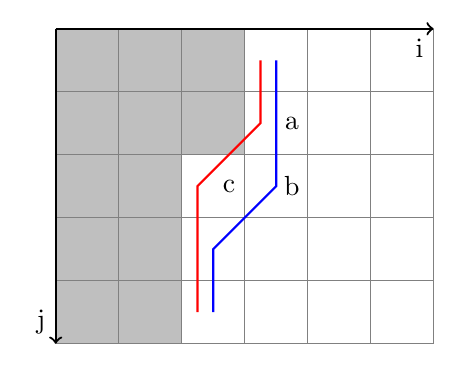
\begin{tikzpicture}
        \fill[lightgray] (0,0) rectangle (1.6,4);
        \fill[lightgray] (0,2.4) rectangle (2.4,4);
        \draw[step=0.8cm,gray,very thin] (0,0) grid (4.8, 4);
        \draw[red, thick] (2.6, 3.6) -- (2.6, 2.8) -- (1.8, 2.0) -- (1.8, 0.4);
        \draw[blue, thick] (2.8, 3.6) -- (2.8, 2.0) -- (2.0, 1.2) -- (2.0, 0.4);
        \node[draw=none] at (3.0, 2.8){a}; 
        \node[draw=none] at (3.0, 2.0){b}; 
        \node[draw=none] at (2.2, 2.0){c}; 
        \draw[thick,->] (0,4) -- (0,0) node[anchor=south east] {j};
        \draw[thick,->] (0,4) -- (4.8,4) node [anchor=north east]{i};
        \end{tikzpicture}
        \end{center}
        \par (註:這裡的 dp 都是 0-base)令$dp[i][j][s]$代表目前已填滿$0$到$i-1$列以及第$i$列的$0$到$j-1$項,且目前的輪廓線上格子填滿的狀態是$s$的方法數。這裡的輪廓線是指第$i+1$列的$0$到$j-1$項以及第$i$列的$j$到$n-1$項共$n$格。用上圖來看的話,目前算好了$dp[3][1]$,那灰色格子都被填滿,紅色(左邊)線段為$s$表示的輪廓線,而我們要算$dp[3][2]$,把輪廓線更新成藍色線段。現在來考慮轉移的方式:
        \begin{itemize}
            \item 用一個骨牌填滿$c, b$,那原本$c$是空的
            \item 用一個骨牌填滿$a, b$,那$a$是空的,$c$必須是滿的
            \item 不用骨牌填滿$b$,那$c$必須是滿的
        \end{itemize}
        \par 這裡的重點就是只考慮$b$要如何填滿,而由前面的分析可以發現,只需要$dp[i][j-1]$裡的狀態就能更新$dp[i][j]$,因此我們可以使用滾動 dp 簡化實作,可以用下面的程式碼加強理解。
        \begin{C++}
        #define mod 1000000007
        int dp[2][1<<10];
        void madd(int &u, int v) { //u = (u + v) % mod
            u += v - mod; u += mod & (u>>31);
        }
        int main() {
            int n, m;
            cin >> n >> m;
            dp[0][(1<<n) - 1] = 1;
            for (int i = 0;i < m;i++) {
                for (int j = 0;j < n;j++) {
                    for (int s = 0;s < (1<<n);s++) {
                        if (!(s & (1<<j))) madd(dp[1][s ^ (1<<j)], dp[0][s]); //case 1
                        if (j && (s & (1<<j)) && (s & (1<<(j-1)))) {
                            madd(dp[1][s], dp[0][s ^ (1<<(j-1))]);
                        } //case 2
                        if (s & (1<<j)) madd(dp[1][s ^ (1<<j)], dp[0][s]); //case 3
                    }
                    for (int s = 0;s < (1<<n);s++) {
                        dp[0][s] = dp[1][s];
                        dp[1][s] = 0;
                    }
                }
            }
            cout << dp[0][(1<<n) - 1] << "\n";
        }
        \end{C++}
        \section{例題}
        \problem{\href{https://tioj.ck.tp.edu.tw/problems/2153}{開窗戶 (TIOJ 2153)}}{
        對於一個$n \times m$的 01 表格,如果每個$2 \times 2$的子矩形(連續)都至少有兩個 1,那麼這個表格是好的。輸出好的表格數模$K$。
        
        $n, m \leq 16, 2\leq K \leq 10^9 + 9$
        }


\section{矩陣快速冪優化}
    在此章節中,筆者是基於讀者對於矩陣的性質有基本的概念(約略為台灣 108 課綱下的數學 A 矩陣一章之內容),因此對於矩陣的基本性質將不多加贅述。

    還記得這份講義的第一題嗎?
    \problem{Fibonacci Sequence 2 (No Judge)}{
        定義費式數列為
        $F_i = \begin{cases}
            1, & \text{if $i \leq 2$}.\\
            F_{i-1} + F_{i-2}, & \text{otherwise}.
        \end{cases}$
        
        求出 $F_n$  ($n \leq 10^{18}$)
    }
    這題實際上可以做到遠比 $O(n)$ 更好的複雜度,那就是透過矩陣快速冪優化。
    
    在許多 $1D/0D$ 問題中,DP 轉移式經常是帶有前常數項的遞迴式(像是費式數列),也因此我們可以將轉移式改寫為一個矩陣,像是費式數列的轉移式若寫成矩陣就是
    $$\begin{bmatrix}
        F_i \\
        F_{i-1}
    \end{bmatrix} = 
    \begin{bmatrix}
    1 & 1 \\
    1 & 0
    \end{bmatrix} \times
    \begin{bmatrix}
    F_{i-1} \\
    F_{i-2}
    \end{bmatrix}
    $$
    
    而我們如果想要快速的求出 $F_n$,可以這樣計算:
    $$\begin{bmatrix}
    F_n \\
    F_n-1
    \end{bmatrix} = 
    \begin{bmatrix}
    1 & 1 \\
    1 & 0
    \end{bmatrix}^{n-2} \times
    \begin{bmatrix}
    F_2 \\
    F_1
    \end{bmatrix}$$
    
    寫成矩陣乘法有什麼好處呢?那就是我們可以使用快速冪來優化。
    
    \theorem{矩陣乘法的結合律}{
        矩陣乘法若可乘,則存在結合律,如:
        $$A \times B \times C = (A \times B) \times C = A \times (B \times C)$$
    }
    
    有了結合律,我們就可以使用快速冪去加速矩陣的次方運算,而矩陣乘法本身若直接用矩陣乘法的定義去計算,複雜度會是 $O(k^3)$ ($k$ 為矩陣大小),因此對於部分題目,我們可以用矩陣快速冪優化到 $O(k^3 \log(n))$,且解決 $k$ 為常數的 1D/0D 題目時複雜度就會是 $O(\log(n))$。
    
    值得注意的是,有些並非傳統矩陣乘法的運算,由於存在結合律,因此可以使用一樣的概念去解決,在下方例題中就有一道這種題目。
    
    \subsection{例題}
        \problem{西洋棋 (2020 北市賽, \href{https://fgiscoj.fg.tp.edu.tw/problem/4460}{fgiscoj 4460})}{
            西洋棋有 $6$ 種棋子:國王、皇后、主教、騎士、城堡、士兵。現在你每種棋子都有無限枚,你想取出洽 $n$ 枚排成一列,並且國王跟皇后都必須洽有偶數枚,共有多少種排法。
            
            $n \leq 10^9$
        }
        \problem{費式數列 (2018 TOI 初選pC, \href{https://tioj.ck.tp.edu.tw/problems/2053}{TIOJ 2053})}{
            給定 $x_1, x_2, a, b$,
            
            定義對於 $i > 2, x_i = bx_{i-1} + ax_{i-2}$ ,計算 $x_n \mod 10^9 + 7$
            
            $0 \leq x_1, x_2, a, b \leq 10^9, 3 \leq n \leq 10^9$
        }
        \problem{城市旅遊問題 (\href{https://tioj.ck.tp.edu.tw/problems/1778}{TIOJ 1778})}{
            在一張 $n$ 個點 $m$ 條邊的無向圖上,求由 $s$ 走到 $t$ 且恰經過 $k$ 條邊的路徑有幾條。
            
            $2 \leq n \leq 100, 0 \leq m \leq 50000, 0 \leq k \leq 10^{15}$
        }
        \problem{大富翁 (\href{https://tioj.ck.tp.edu.tw/problems/2151}{TIOJ 2151})}{}

\section{DP 與其他概念的結合}

\section{技巧}
    \subsection{滾動}
    \subsection{回朔}

\section{後記}
    DP 是一個非常大的章節,以上技巧雖然已足夠拿到 APCS 5級分或多數競賽題目,但各種 DP 優化技巧往往是最後決勝的關鍵。
    
\end{document}
